\section {Análisis espacial de los resultados}

Los datos obtenidos mediante el simulador del proceso evolutivo, contienen información que nos
permiten analizarlos en el contexto de un SIG, para identificar los focos de infestación mediante
técnicas de interpolación espacial.

Los niveles de riesgos fueron determinados de acuerdo a los tipos de zonas determinados en la
\secref{subsec:cap4-zonificacion}. Se consideran de mayor riesgo las zonas propicias para el
desarrollo del Aedes aegypti. En la \tabref{tab:niveles-riesgo-zonas}, se presentan los niveles de
riesgo definidos según la \tabref{tab:cap4-puntaje-zona}.


\begin{table}[!hptb]
    \begin{minipage}{\textwidth}
\begin{center}
    \caption{\label{tab:niveles-riesgo-zonas} Niveles de infestación de las zonas.}
    \begin{tabular}{p{3cm} l c c c}
        \hline \\
         Niveles de  & Color & Mínimo$^a$ & Máximo$^a$ \\
         infestación & identificador & $u(x,y)$   & $u(x,y)$  \\
        \hline
        \hline\\
        Muy bajo  & \cellcolor{muybajo}& 0  & 19 \\
        Bajo    & \cellcolor{bajo}& 20 & 35 \\
        Normal & \cellcolor{normal}& 36 & 51 \\
        Alto   & \cellcolor{alto}& 52 & 69 \\
        Muy Alto & \cellcolor{muyalto} & 70 & --$^b$\\
    \end{tabular}
    \footnotetext[1]{Rango mínimo y máximo de $u(x,y)$ permitido para el tipo de zona.}
    \footnotetext[2]{No se estableció un límite superior para este nivel. }
\end{center}
    \end{minipage}
\end{table}

\subsection{Análisis general de la población}
La distribución geográfica, dispersión y niveles de infestación de las poblaciones de Aedes aegypti
son presentadas como mapas de interpolación, donde para la interpolación espacial fueron
seleccionados los individuos pertenecientes a las poblaciones correspondientes a un día del
periodo de simulación. Para el análisis espacial fueron seleccionadas los datos obtenidos mediante
la simulación del proceso evolutivo a 6 temperaturas constantes(15 a 34 \textcelsius). Los días
del periodo de simulación, utilizados para generar los mapas de interpolación, fueron
seleccionados teniendo en cuenta el crecimiento y decrecimiento de la población observado en
la \figref{fig:desarrollo-poblacion-all} con el fin de resaltar los eventos más relevantes de cada
población.

\begin{figure}[!htbp]
    \centering
    \begin{subfigure}[b]{0.45\textwidth}
            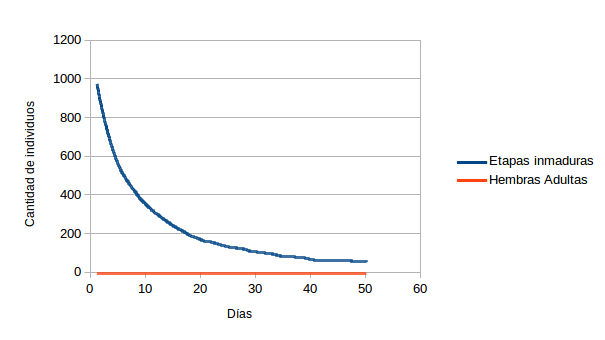
\includegraphics[width=\textwidth]{capitulo-6/graphics/desarrollo-poblacion-15.png}
            \caption{\label{fig:desarrollo-poblacion-15}Población a 15 \textcelsius.}
    \end{subfigure}
    ~~~~
    \begin{subfigure}[b]{0.45\textwidth}
            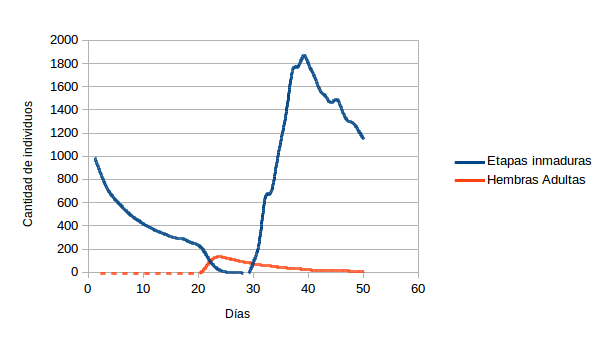
\includegraphics[width=\textwidth]{capitulo-6/graphics/desarrollo-poblacion-20.png}
            \caption{\label{fig:desarrollo-poblacion-20}Población a 20 \textcelsius.}
    \end{subfigure}

    \begin{subfigure}[b]{0.45\textwidth}
            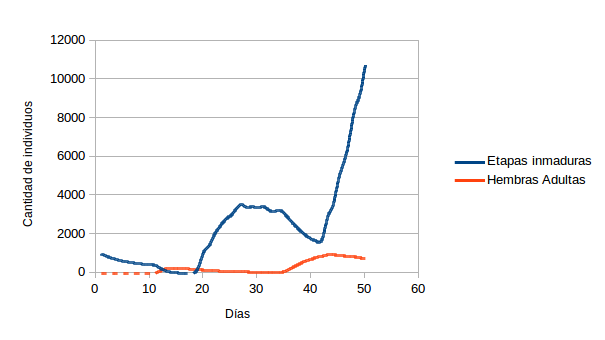
\includegraphics[width=\textwidth]{capitulo-6/graphics/desarrollo-poblacion-24.png}
            \caption{\label{fig:desarrollo-poblacion-24}Población a 24 \textcelsius.}
    \end{subfigure}
    ~~~~
    \begin{subfigure}[b]{0.45\textwidth}
            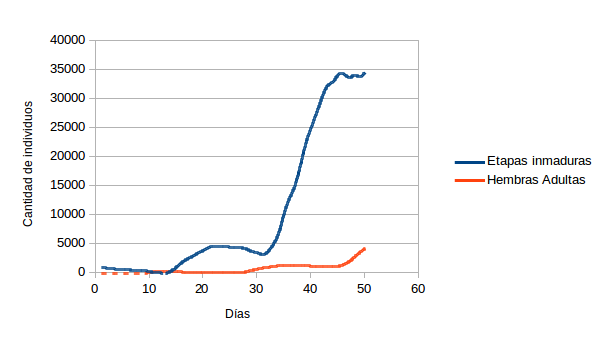
\includegraphics[width=\textwidth]{capitulo-6/graphics/desarrollo-poblacion-27.png}
            \caption{\label{fig:desarrollo-poblacion-27}Población a 27 \textcelsius.}
    \end{subfigure}

    \begin{subfigure}[b]{0.45\textwidth}
            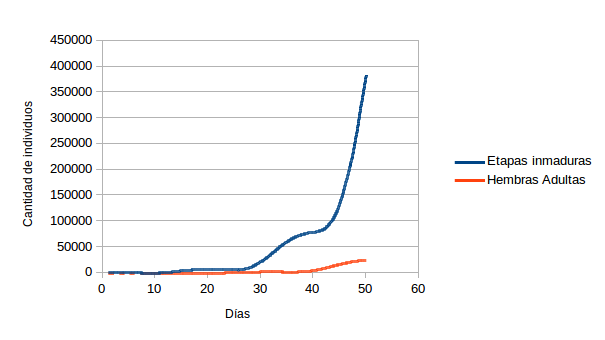
\includegraphics[width=\textwidth]{capitulo-6/graphics/desarrollo-poblacion-30.png}
            \caption{\label{fig:desarrollo-poblacion-30}Población a 30 \textcelsius.}
    \end{subfigure}
    ~~~~
    \begin{subfigure}[b]{0.45\textwidth}
            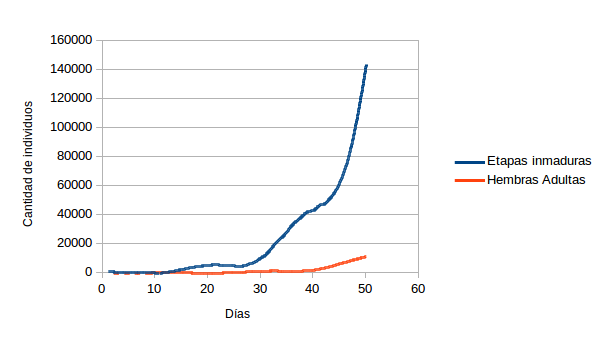
\includegraphics[width=\textwidth]{capitulo-6/graphics/desarrollo-poblacion-34.png}
            \caption{\label{fig:desarrollo-poblacion-34}Población a 34 \textcelsius.}
    \end{subfigure}

    \caption{\label{fig:desarrollo-poblacion-all} Análisis del comportamiento de la población de mosquitos en relación al tiempo a 6 temperaturas constantes (15-34 \textcelsius).}
\end{figure}

En la \figref{fig:desarrollo-poblacion-all}, se pueden observar el comportamiento de las
poblaciones a 6 temperaturas constantes (15-34 \textcelsius). En general, para todos los casos, la
población inicial sufre un decrecimiento causada por la mortalidad diaria de los individuos a
temperaturas entre 15 y 34 \textcelsius, y por la emergencia de adultos a temperaturas entre 20 y
34 \textcelsius. La aparición de adultos implica que la población de individuos en etapas
inmaduras (huevos, larvas y pupas), llegaron a completar su ciclo de desarrollo para dar lugar a
mosquitos adultos, por lo tanto la población de individuos en etapas inmaduras tiende a disminuir
y mientras que la población de mosquitos adultos tiende a aumentar. El crecimiento de la población
se debe a que las hembras adultas pertenecientes a la población de mosquitos, culminaron su ciclo
gonotrófico y dieron lugar la ovipostura.

En la \secref{sec:tasas-desarrollo-mortalidad} se presentaron las tasas de desarrollo obtenidas a
diferentes temperaturas, en donde se pudo observar que a medida que la temperatura aumenta, las
tasas de desarrollo son menores, motivo por el cual las poblaciones de individuos en etapas
inmaduras, sometidos a temperaturas más elevadas, tienden a disminuir su tamaño rápidamente debido
a que se desarrollan con mayor rapidez, dando lugar a su etapa de adulto. Del mismo modo el ciclo
gonotrófico, presentado en la \secref{sec:tasa-ciclo-gonotrofico}, para las hembras adultas
tienden a disminuir su duración, causando que el intervalo entre oviposturas disminuya, en
consecuencia el tamaño de la población de individuos en etapas inmaduras aumenta rápidamente.

Todas las poblaciones, sometidas a temperaturas que permitieron la aparición de adultos,
experimentaron una dispersión hacia el noreste debido a que la dirección del viento utilizada era
de sureste.
%Tendencia de dispersión causada porque la dirección del viento es suroeste

%Solo las hembras adultas se muestran que representa el 50\% de la población

\subsection{Análisis de la población a 15 \textcelsius}
%Población a 15 C
En la \figref{fig:desarrollo-poblacion-15}, se puede apreciar que el tamaño de la población a 15
\textcelsius, tiende a disminuir con el transcurrir del tiempo. Considerando que el estado inicial
de los individuos, para la simulación del proceso evolutivo, es el de larva, tenemos una tasa de
desarrollo igual a $44,33$ días de desarrollo
(\tabref{tab:desarrollo-larva-rueda1990temperature-test}), para las larvas.

\begin{figure}[!htbp]
    \centering
    \begin{subfigure}[b]{0.45\textwidth}
            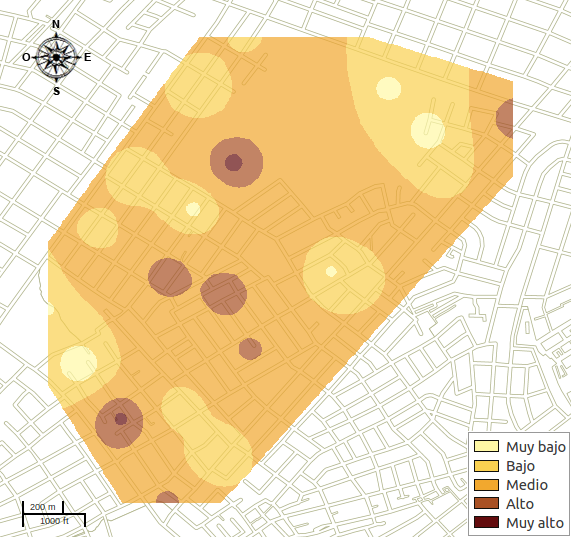
\includegraphics[width=\textwidth]{capitulo-6/graphics/raster/temp-15-0.png}
            \caption{\label{fig:niveles-infestacion-15-a}Primer día de simulación.}
    \end{subfigure}
    ~~
    \begin{subfigure}[b]{0.45\textwidth}
            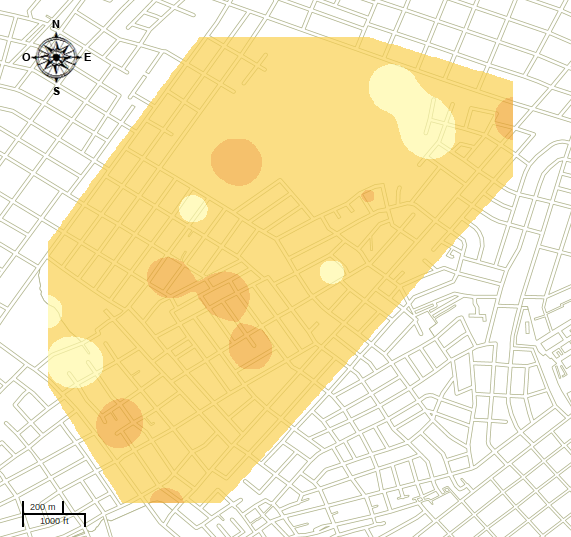
\includegraphics[width=\textwidth]{capitulo-6/graphics/raster/temp-15-2.png}
            \caption{\label{fig:niveles-infestacion-15-b}Día número 3 de simulación.}
    \end{subfigure}
    \begin{subfigure}[b]{0.45\textwidth}
            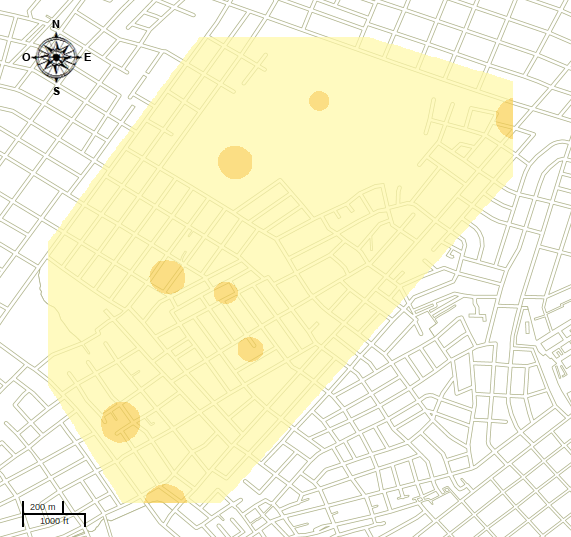
\includegraphics[width=\textwidth]{capitulo-6/graphics/raster/temp-15-7.png}
            \caption{\label{fig:niveles-infestacion-15-c}Día número 8 de simulación.}
    \end{subfigure}
    ~~
    \begin{subfigure}[b]{0.45\textwidth}
            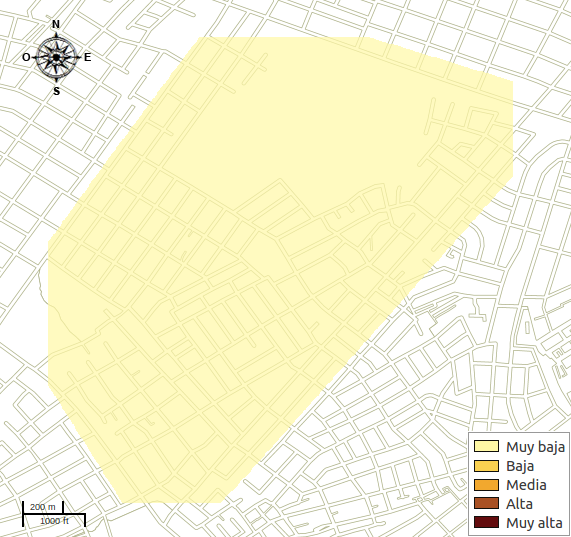
\includegraphics[width=\textwidth]{capitulo-6/graphics/raster/temp-15-9.png}
            \caption{\label{fig:niveles-infestacion-15-d}Día número 10 de simulación.}
    \end{subfigure}
    \caption{\label{fig:niveles-infestacion-15} Mapas de interpolación de la población correspondientes a los días 1, 3, 8 y 10 de simulación a 15 \textcelsius.}
\end{figure}

En un periodo de 50 días a 15 \textcelsius, no se pueden observar mosquitos adultos motivo por el
cual la población tiende a disminuir su tamaño y por ende el riesgo de infestación del área de
estudio. En la \figref{fig:niveles-infestacion-15} se puede observar el rápido decrecimiento de la
población y de los niveles de infestación. Para el octavo día, en la
\figref{fig:niveles-infestacion-15-c}, se puede apreciar el rápido decrecimiento en los niveles de
infestación, debido a la disminución de la población observados en
\figref{fig:desarrollo-poblacion-15}. A partir del décimo día,
\figref{fig:niveles-infestacion-15-d}, los niveles de infestación se mantienen constantemente
bajos, por lo que los mapas de interpolación se mantienen constantes hasta el final del periodo de
simulación.

Debido a que no se pudieron observar adultos la población inicial no sufrió ninguna dispersión, ya
que las etapas inmaduras del mosquito son etapas acuáticas.

\subsection{Análisis de la población a 20\textcelsius}
%Población a 20 C
En la \figref{fig:desarrollo-poblacion-20}, se puede observar el comportamiento de la población a
20 \textcelsius, en donde la población de individuos en sus etapas inmaduras va decreciendo hasta
desaparecer temporalmente el día 28, no así la población de adultos. En la
\figref{fig:niveles-infestacion-20-b}, se puede observar que no existen mosquitos en sus etapas
inmaduras, para generar un mapa de interpolación del área, sin embargo se pueden observar la
distribución geográfica de las hembras adultas. Desde el día 21, en la
\figref{fig:desarrollo-poblacion-20}, comienzan a observarse los primeros mosquitos adultos, que a
partir del día 30, las hembras adultas, comienzan oviponer, generando la reaparición de la
población de mosquitos que alcanza su máximo valor en el día 39.

\begin{figure}[!htbp]
    \centering
    \begin{subfigure}[b]{0.45\textwidth}
            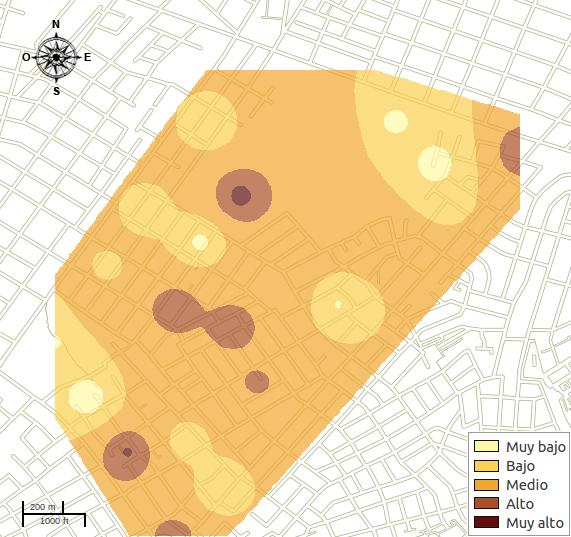
\includegraphics[width=\textwidth]{capitulo-6/graphics/raster/temp-20-0.png}
            \caption{\label{fig:niveles-infestacion-20-a}Primer día de simulación.}
    \end{subfigure}
    ~~
    \begin{subfigure}[b]{0.45\textwidth}
            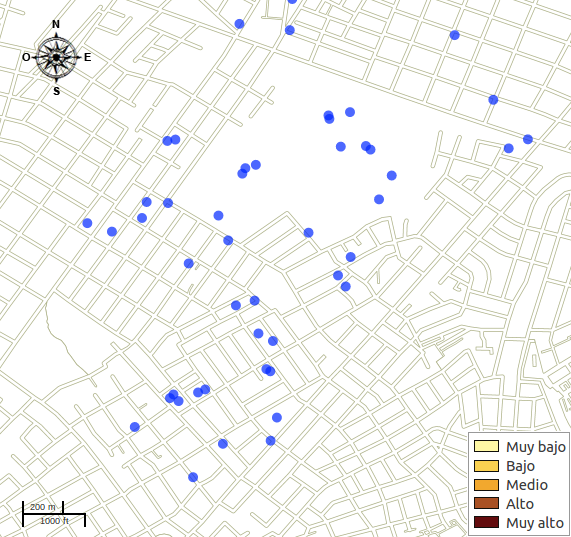
\includegraphics[width=\textwidth]{capitulo-6/graphics/raster/temp-20-28.png}
            \caption{\label{fig:niveles-infestacion-20-b}Día número 28 de simulación.}
    \end{subfigure}

    \begin{subfigure}[b]{0.45\textwidth}
            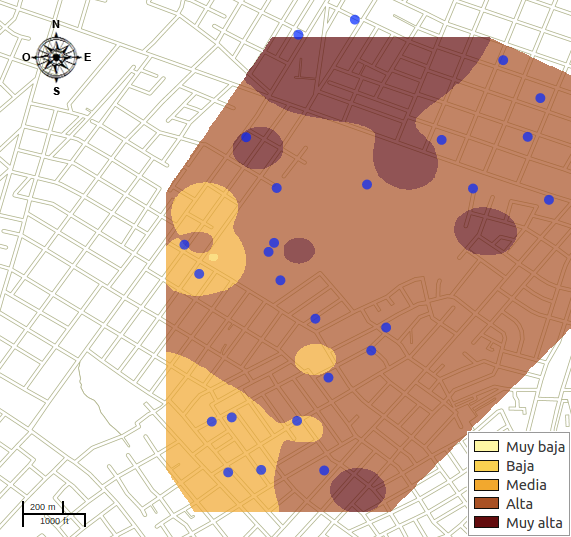
\includegraphics[width=\textwidth]{capitulo-6/graphics/raster/temp-20-35.png}
            \caption{\label{fig:niveles-infestacion-20-c}Día número 36 de simulación.}
    \end{subfigure}
    ~~
    \begin{subfigure}[b]{0.45\textwidth}
            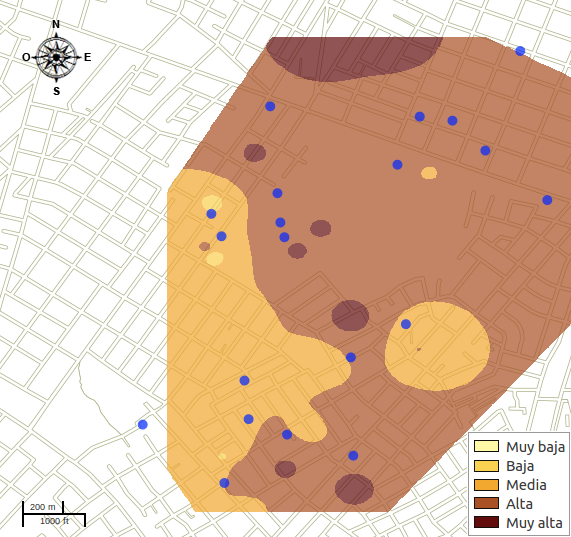
\includegraphics[width=\textwidth]{capitulo-6/graphics/raster/temp-20-38.png}
            \caption{\label{fig:niveles-infestacion-20-d}Día número 39 de simulación.}
    \end{subfigure}

    \caption{\label{fig:niveles-infestacion-20} Mapas de interpolación de la población correspondientes a los días 1, 29, 36 y 39 de simulación a 20 \textcelsius, y la distribución de las hembras adultas (puntos en azul). }
\end{figure}

En la \figref{fig:niveles-infestacion-20} se puede apreciar los niveles de infestación para los
días 1, 28, 36 y 38 del periodo de simulación. Además se observa el desplazamiento de los focos de
infestación, causado por la dispersión de los adultos, que pasan de su estado inicial
(\figref{fig:niveles-infestacion-20-a}), a generar nuevos focos
(\figref{fig:niveles-infestacion-20-c} y \figref{fig:niveles-infestacion-20-d}). Cabe resaltar
que, un aumento en el tamaño de la población no necesariamente implica mayores niveles de
infestación. Esto se puede observar realizando una comparación entre los niveles de infestación
presentados en las \figref{fig:niveles-infestacion-20-c} y \figref{fig:niveles-infestacion-20-d},
y el tamaño de la población para los días 36 y 39 del periodo de simulación, en donde el día 39
cuenta con una población de mayor tamaño que el día 36, pero en este último se observan mayores
niveles de infestación. Esto se debe a que los mapas de interpolación dependen de la distribución
geográfica de los individuos de la población y la concentración de los mismos en $(x,y)$.

A 20 \textcelsius se observa el desplazamiento de los focos de infestación en dirección al
noreste, debido a que la dirección del viento utilizada es igual al sureste y los mosquitos
adultos tienden a volar en dirección contraria al viento. Este desplazamiento se puede observar en
las figuras \figref{fig:niveles-infestacion-20-a}, \figref{fig:niveles-infestacion-20-c} y
\figref{fig:niveles-infestacion-20-d}.

\subsection{Análisis de la población a 24\textcelsius}
%Población a 24 C
En la \figref{fig:desarrollo-poblacion-24}, se puede observar el comportamiento de la población a
24 \textcelsius, en donde la población de individuos en sus etapas inmaduras va decreciendo hasta
desaparecer temporalmente el día 17. A partir del día 12, en la
\figref{fig:desarrollo-poblacion-24}, pueden observarse los primeros mosquitos adultos, donde a
partir del día 19 las hembras adultas, comienzan oviponer, generando la reaparición de la
población de mosquitos, alcanzando 2 picos importantes en día 27 y 50.

\begin{figure}[!htbp]
    \centering
    \begin{subfigure}[b]{0.45\textwidth}
            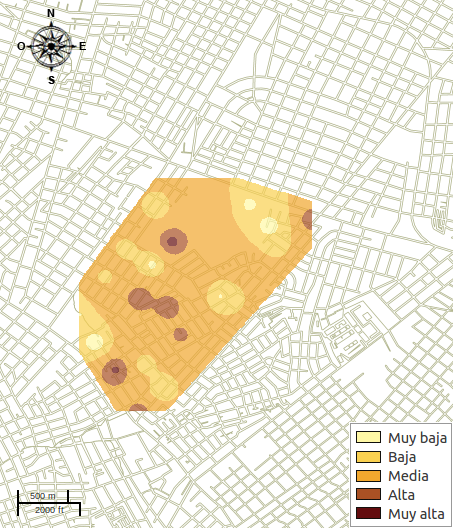
\includegraphics[width=\textwidth]{capitulo-6/graphics/raster/temp-24-0.png}
            \caption{\label{fig:niveles-infestacion-24-a}Primer día de simulación.}
    \end{subfigure}
    ~~
    \begin{subfigure}[b]{0.45\textwidth}
            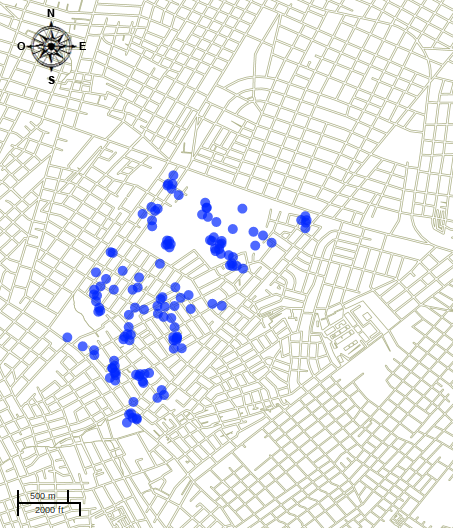
\includegraphics[width=\textwidth]{capitulo-6/graphics/raster/temp-24-16.png}
            \caption{\label{fig:niveles-infestacion-24-b}Día número 17 de simulación.}
    \end{subfigure}

    \begin{subfigure}[b]{0.45\textwidth}
            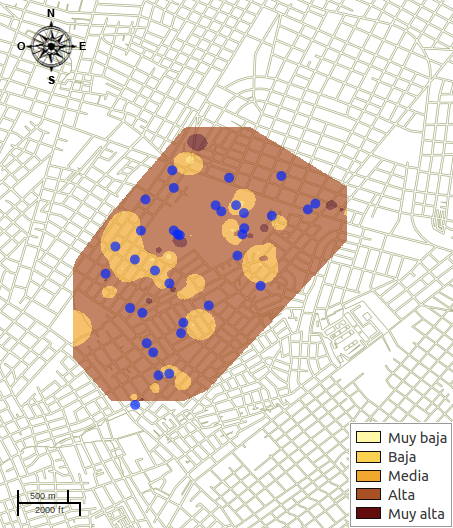
\includegraphics[width=\textwidth]{capitulo-6/graphics/raster/temp-24-26.png}
            \caption{\label{fig:niveles-infestacion-24-c}Día número 27 de simulación.}
    \end{subfigure}
    ~~
    \begin{subfigure}[b]{0.45\textwidth}
            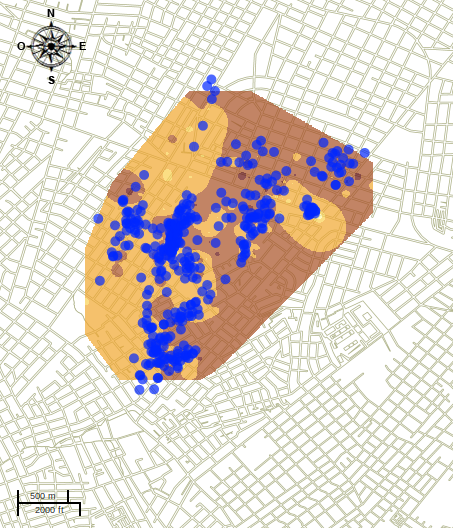
\includegraphics[width=\textwidth]{capitulo-6/graphics/raster/temp-24-49.png}
            \caption{\label{fig:niveles-infestacion-24-d}Día número 50 de simulación.}
    \end{subfigure}

    \caption{\label{fig:niveles-infestacion-24} Mapas de interpolación de la población correspondientes a los días 1, 17, 27 y 50 de simulación a 24 \textcelsius, y la distribución de las hembras adultas (puntos en azul). }
\end{figure}

En la \figref{fig:niveles-infestacion-24-b}, se puede observar que no existen mosquitos en sus
etapas inmaduras, para generar un mapa de interpolación del área, sin embargo se pueden observar la
distribución geográfica de las hembras adultas.

En la \figref{fig:niveles-infestacion-24} se puede observar los niveles de infestación para los
días 1, 17, 27 y 50 del periodo de simulación. En general, se observa el desplazamiento de los
focos de infestación en dirección al noreste, debido a que la dirección del viento utilizada es
igual al sureste y los mosquitos adultos tienden a volar en dirección contraria al viento. Este
desplazamiento se puede observar en las figuras
 \figref{fig:niveles-infestacion-24-a}, \figref{fig:niveles-infestacion-24-c} y
\figref{fig:niveles-infestacion-24-d}.

\subsection{Análisis de la población a 27\textcelsius}
%Población a 27 C
En la \figref{fig:desarrollo-poblacion-27}, se puede observar el comportamiento de la población a
27 \textcelsius, en donde la población de individuos en sus etapas inmaduras va decreciendo hasta
alcanzar un total de 8 individuos en etapas inmaduras en el día 13. A partir del día 10, en la
\figref{fig:desarrollo-poblacion-27}, pueden observarse los primeros mosquitos adultos, donde a
partir del día 14 las hembras adultas, comienzan oviponer, generando un crecimiento de la
población de mosquitos, alcanzando 2 picos importantes en día 24 y 50.

\begin{figure}[!htbp]
    \centering
    \begin{subfigure}[b]{0.45\textwidth}
            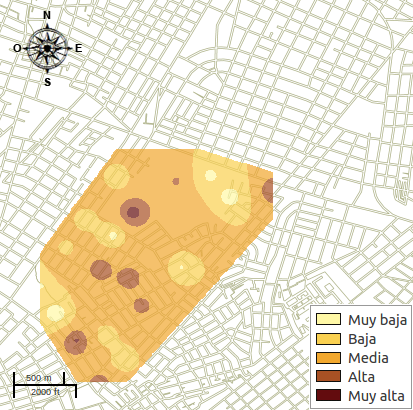
\includegraphics[width=\textwidth]{capitulo-6/graphics/raster/temp-27-0.png}
            \caption{\label{fig:niveles-infestacion-27-a}Primer día de simulación.}
    \end{subfigure}
    ~~
    \begin{subfigure}[b]{0.45\textwidth}
            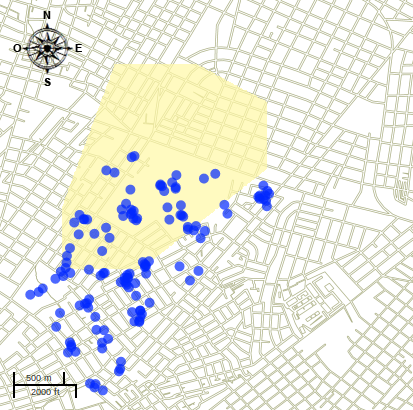
\includegraphics[width=\textwidth]{capitulo-6/graphics/raster/temp-27-12.png}
            \caption{\label{fig:niveles-infestacion-27-b}Día número 13 de simulación.}
    \end{subfigure}

    \begin{subfigure}[b]{0.45\textwidth}
            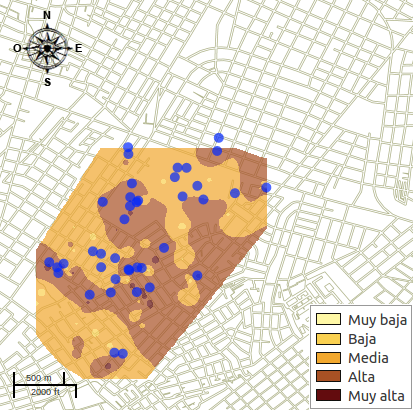
\includegraphics[width=\textwidth]{capitulo-6/graphics/raster/temp-27-22.png}
            \caption{\label{fig:niveles-infestacion-27-c}Día número 23 de simulación.}
    \end{subfigure}
    ~~
    \begin{subfigure}[b]{0.45\textwidth}
            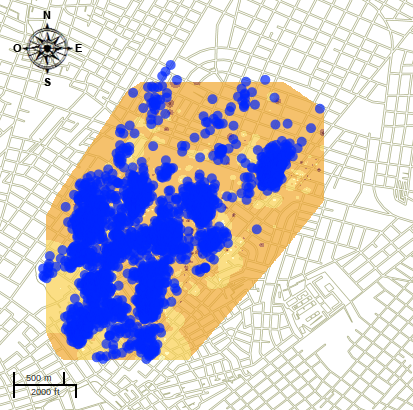
\includegraphics[width=\textwidth]{capitulo-6/graphics/raster/temp-27-49.png}
            \caption{\label{fig:niveles-infestacion-27-d}Día número 50 de simulación.}
    \end{subfigure}

    \caption{\label{fig:niveles-infestacion-27} Mapas de interpolación de la población correspondientes a los días 1, 13, 23 y 50 de simulación a 27 \textcelsius, y la distribución de las hembras adultas (puntos en azul). }
\end{figure}

En la \figref{fig:niveles-infestacion-27-b}, se puede apreciar un nivel de infestación bajo, sin
embargo se puede observar la distribución geográfica de las hembras adultas, lo que implica que la
disminución de la población de mosquitos en sus etapas inmaduras no solo se encuentra influenciada
por la mortalidad diaria, sino también por la aparición de mosquitos adultos producto de la culminación de el ciclo de desarrollo de los mosquitos en etapas inmaduras.

En la \figref{fig:niveles-infestacion-27} se puede observar los niveles de infestación
para los días 1, 12, 22 y 50 del periodo de simulación. En general, se observa el
desplazamiento de los focos de infestación en dirección al noreste, debido a que la dirección del
viento utilizada es igual al sureste y los mosquitos adultos tienden a volar en dirección
contraria al viento. Este desplazamiento se puede observar en las figuras
\figref{fig:niveles-infestacion-27-a},\figref{fig:niveles-infestacion-27-b},
\figref{fig:niveles-infestacion-27-c} y \figref{fig:niveles-infestacion-27-d}.

\subsection{Análisis de la población a 30\textcelsius}
%Población a 30 C
En la \figref{fig:desarrollo-poblacion-30}, se puede observar el comportamiento de la población a
30 \textcelsius, en donde la población de individuos en sus etapas inmaduras va decreciendo hasta
alcanzar un total de 39 individuos en etapas inmaduras en el día 10. A partir del día 8, en la
\figref{fig:desarrollo-poblacion-30}, pueden observarse los primeros mosquitos adultos, donde a
partir del día 11 las hembras adultas, comienzan oviponer, generando un crecimiento de la
población de mosquitos, alcanzando 2 picos importantes en día 21 y 50.

\begin{figure}[!htbp]
    \centering
    \begin{subfigure}[b]{0.45\textwidth}
            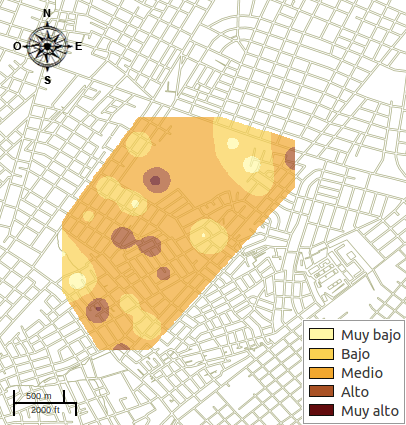
\includegraphics[width=\textwidth]{capitulo-6/graphics/raster/temp-30-0.png}
            \caption{\label{fig:niveles-infestacion-30-a}Primer día de simulación.}
    \end{subfigure}
    ~~
    \begin{subfigure}[b]{0.45\textwidth}
            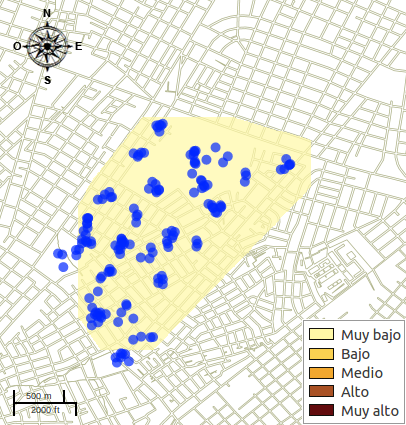
\includegraphics[width=\textwidth]{capitulo-6/graphics/raster/temp-30-9.png}
            \caption{\label{fig:niveles-infestacion-30-b}Día número 10 de simulación.}
    \end{subfigure}

    \begin{subfigure}[b]{0.45\textwidth}
            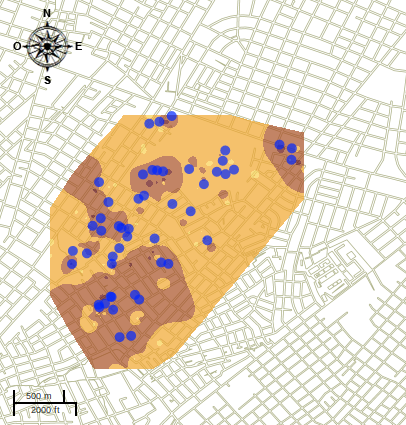
\includegraphics[width=\textwidth]{capitulo-6/graphics/raster/temp-30-20.png}
            \caption{\label{fig:niveles-infestacion-30-c}Día número 21 de simulación.}
    \end{subfigure}
    ~~
    \begin{subfigure}[b]{0.45\textwidth}
            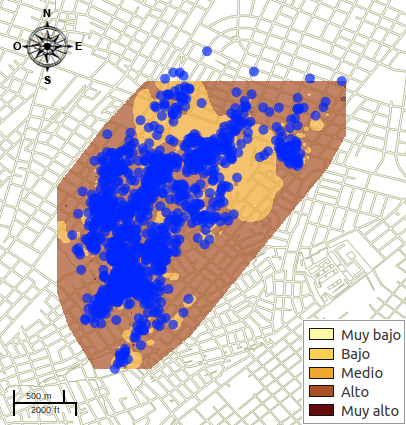
\includegraphics[width=\textwidth]{capitulo-6/graphics/raster/temp-30-35.png}
            \caption{\label{fig:niveles-infestacion-30-d}Día número 50 de simulación.}
    \end{subfigure}

    \caption{\label{fig:niveles-infestacion-30} Mapas de interpolación de la población correspondientes a los días 1, 10, 21 y 35 de simulación a 30 \textcelsius, y la distribución de las hembras adultas (puntos en azul). }
\end{figure}

En la \figref{fig:niveles-infestacion-30-b}, se puede apreciar un nivel de infestación bajo, sin
embargo se puede observar la distribución geográfica de las hembras adultas, lo que implica que la
disminución de la población de mosquitos en sus etapas inmaduras no solo se encuentra influenciada
por la mortalidad diaria, sino también por la aparición de mosquitos adultos producto de la culminación de el ciclo de desarrollo de los mosquitos en etapas inmaduras.

En la \figref{fig:niveles-infestacion-30} se puede apreciar los niveles de infestación
para los días 1, 10, 21 y 35 del periodo de simulación. En general, se observa el
desplazamiento de los focos de infestación en dirección al noreste, debido a que la dirección del
viento utilizada es igual al sureste y los mosquitos adultos tienden a volar en dirección
contraria al viento. Este desplazamiento se puede observar en las figuras
\figref{fig:niveles-infestacion-30-a},\figref{fig:niveles-infestacion-30-b},
\figref{fig:niveles-infestacion-30-c} y \figref{fig:niveles-infestacion-30-d}.

\subsection{Análisis de la población a 34\textcelsius}
%Población a 34 C
En la \figref{fig:desarrollo-poblacion-34}, se puede observar el comportamiento de la población a
34 \textcelsius, en donde la población de individuos en sus etapas inmaduras va decreciendo hasta
alcanzar un total de 49 individuos en etapas inmaduras en el día 11. A partir del día 9, en la
\figref{fig:desarrollo-poblacion-34}, pueden observarse los primeros mosquitos adultos, donde a
partir del día 12 las hembras adultas, comienzan oviponer, generando un crecimiento de la
población de mosquitos, alcanzando 2 picos importantes en día 21 y 50.

\begin{figure}[!htbp]
    \centering
    \begin{subfigure}[b]{0.45\textwidth}
            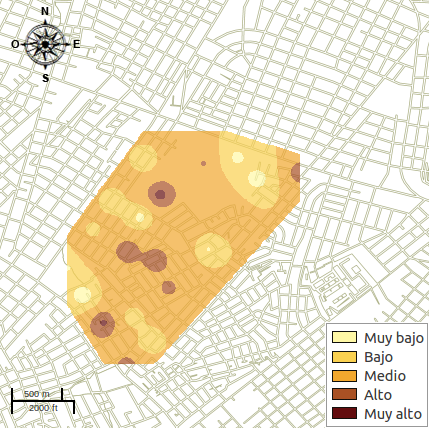
\includegraphics[width=\textwidth]{capitulo-6/graphics/raster/temp-34-0.png}
            \caption{\label{fig:niveles-infestacion-34-a}Primer día de simulación.}
    \end{subfigure}
    ~~
    \begin{subfigure}[b]{0.45\textwidth}
            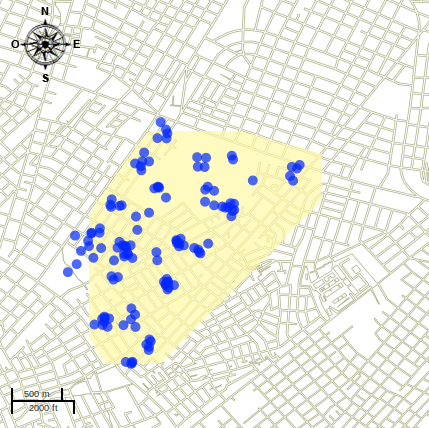
\includegraphics[width=\textwidth]{capitulo-6/graphics/raster/temp-34-10.png}
            \caption{\label{fig:niveles-infestacion-34-b}Día número 11 de simulación.}
    \end{subfigure}

    \begin{subfigure}[b]{0.45\textwidth}
            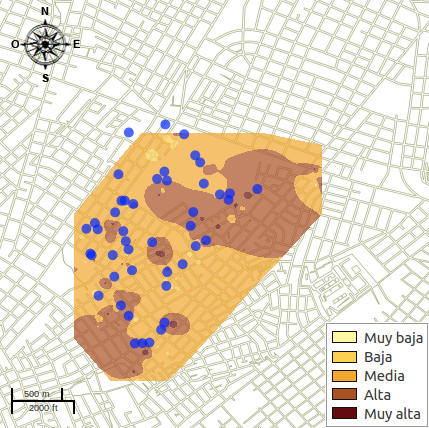
\includegraphics[width=\textwidth]{capitulo-6/graphics/raster/temp-34-20.png}
            \caption{\label{fig:niveles-infestacion-34-c}Día número 21 de simulación.}
    \end{subfigure}
    ~~
    \begin{subfigure}[b]{0.45\textwidth}
            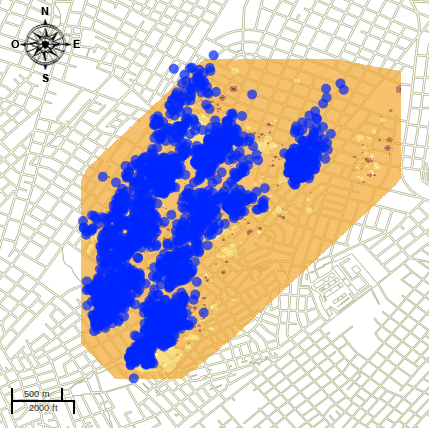
\includegraphics[width=\textwidth]{capitulo-6/graphics/raster/temp-34-42.png}
            \caption{\label{fig:niveles-infestacion-34-d}Día número 43 de simulación.}
    \end{subfigure}

    \caption{\label{fig:niveles-infestacion-34} Mapas de interpolación de la población correspondientes a los días 1, 11, 21 y 43 de simulación a 34 \textcelsius, y la distribución de las hembras adultas (puntos en azul). }
\end{figure}

En la \figref{fig:niveles-infestacion-34-b}, se puede apreciar un nivel de infestación bajo, sin
embargo se puede observar la distribución geográfica de las hembras adultas, lo que implica que la
disminución de la población de mosquitos en sus etapas inmaduras no solo se encuentra influenciada
por la mortalidad diaria, sino también por la aparición de mosquitos adultos producto de la
culminación de el ciclo de desarrollo de los mosquitos en etapas inmaduras.

En la \figref{fig:niveles-infestacion-34} se puede apreciar los niveles de infestación
para los días 1, 11, 21 y 43  del periodo de simulación. En general, se observa el
desplazamiento de los focos de infestación en dirección al noreste, debido a que la dirección del
viento utilizada es igual al sureste y los mosquitos adultos tienden a volar en dirección
contraria al viento. Este desplazamiento se puede observar en las figuras
\figref{fig:niveles-infestacion-34-a},\figref{fig:niveles-infestacion-34-b},
\figref{fig:niveles-infestacion-34-c} y \figref{fig:niveles-infestacion-34-d}.
